
\chapter{Description de l'API de \PpFf}
\label{description.chap}




\begin{figure}
\centering
     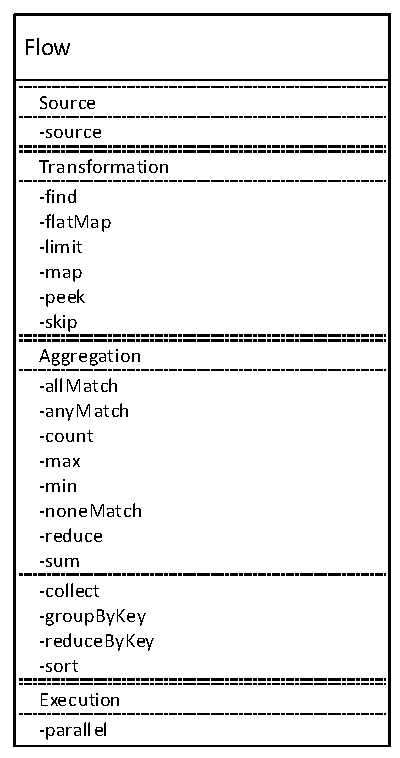
\includegraphics[height=18cm, width=10cm]{Figures/MethodsAPI.pdf}
      \caption{Les diff\'erentes m\'ethodes export\'ees par l'{API} de \ppff,
     regroup\'ees selon leur type de fonctionnalit\'e.}
       \label{MethodesAPI.fig}
\end{figure}



Ce chapitre pr\'esente l'API de la biblioth\`eque \ppff,  c'est-\`a-dire, l'interface avec laquelle interagit le d\'eveloppeur. La conception de l'API de \ppff{} permet aux utilisateurs de tirer parti de la simplicit\'e d'utilisation tout en cachant la complexit\'e des m\'ecanismes concurrents utilis\'es. La figure~\ref{MethodesAPI.fig} pr\'esente une vue d'ensemble des diverses m\'ethodes export\'ees par \ppff. Sur la base du type de fonctionnalit\'e export\'ee, l'API se divise en quatre cat\'egories :  \TT{Source} (Sect.~\ref{source.sect}), \TT{Transformation} (Sect.~\ref{transformation.sect}),  \TT{Aggregation} (Sect.~\ref{aggregation.sect}) et \TT{Execution} (Sect.~\ref{execution.sect}). Quant \`a la cat\'egorie \TT{Aggregation}, elle est elle-m\^eme divis\'ee deux sous-cat\'egories, selon le type de r\'esultat produit~: valeur simple (par ex., r\'esultat bool\'een ou entier) ou collection.

Le chapitre pr\'esente \'egalement le code source d'un exemple, \TT{WordCount}, pour illustrer l'utilisation de l'API et l'effet des principales m\'ethodes --- exemple semblable à celui présenté dans l'article ayant popularisé l'approche \TT{MapReduce}~\citep{DeanGhe04}.

La biblioth\`eque \PpFf{} est impl\'ement\'ee au-dessus de la biblioth\`eque \TT{FastFlow}, impl\'ementation qui sera d\'ecrite au prochain chapitre.



\section{Exemple~: l'application \TT{WordCount}}
\label{descriptionWordCount.sect}


\begin{lstlisting}[
label={wordcount.c++},
language=c++,
caption={Les extraits du code source de l'application \TT{WordCount} qui compte le nombre d'occurrences des mots dans un texte.},
frame=single,
float]
    // ...
    typedef std::vector<std::string> Words;
    Reducer<std::string, int> reducer(
             0, 
             [](int count, std::string _) { return count + 1; },
             std::plus<int>{}
           );

    std::unordered_map<std::string, int> currentResult = 
        Flow
        ::source(inputFile)
        .parallel(4)
        .flatMap<std::string, Words, std::string>(splitInWords)			
        .map<std::string, std::string>(toLowercaseLetters)			
        .reduceByKey<std::string, std::string, int>(reducer); 
    // ...
\end{lstlisting}

L'application \TT{WordCount} pr\'esent\'ee dans ce chapitre illustre le fonctionnement de \TT{PpFf}. Les extraits du code source de l'application sont donn\'e dans le listing~\ref{wordcount.c++}. L'application compte le nombre d'occurrences des mots dans un fichier texte. Cette application est compos\'ee en combinant plusieurs op\'erations.



\goodbreak
Les op\'erations d\'efinissant le pipeline sont les suivantes :
\begin{itemize}

\item  La premi\`ere op\'eration d'un pipeline sert \`a d\'efinir la \emph{source} du flux de donn\'ees. Ici, la source est
constitu\'ee par les lignes contenues dans un fichier. C'est la
m\'ethode statique \TT{source()} qui permet d'extraire et retourner un
flux avec les lignes du fichier. Le fichier est sp\'ecifi\'e par un nom de fichier
(une chaine, \TT{inputFile}) fourni en argument \`a la m\'ethode
\TT{source}.


\item L'appel \`a \TT{parallel(4)} permet de r\'epartir les \'el\'ements du flux entre divers \emph{threads} --- ici, quatre (4) \emph{threads} --- et donc d'ex\'ecuter les \'etapes qui suivent en parall\`ele. 



\item L'op\'eration \TT{flatMap} d\'ecompose chaque ligne en mots individuels en appliquant la fonction \TT{splitInWords} sur chacune des lignes.

\item L'op\'eration \TT{map} transforme chacun des mots en rempla\c{c}ant les lettres majuscules d'un mot en lettres minuscules en appliquant la fonction \TT{toLowercaseLetters}.

\item Finalement, l'op\'eration \TT{reduceByKey}  regroupe les mots similaires ensemble et compte le nombre d'occurrences de chaque mot, et ce par l'utilisation du \TT{Reducer} (cf.~Sect.~\ref{reducer.sect}).
\end{itemize}


\section{Flux de donn\'ees: type \TT{Flow}}

L'interface propos\'ee en \TT{PpFf} consiste en un ensemble de m\'ethodes qui permettent \`a l'utilisateur de manipuler des flux de donn\'ees de mani\`ere simple et efficace. L'interface s'inspire de celle introduite pour les \TT{Stream}s de \TT{Java} 8. L'annexe~\ref{methodes-api.ann} d\'ecrit bri\`evement les m\'ethodes export\'ees par l'API, regroup\'ees selon leur fonctionnalit\'e, puis en ordre alphab\'etique \`a l'int\'erieur d'une cat\'egorie.



Comme on peut le voir dans le tableau~\ref{methodes-api.ann}, la d\'eclaration des m\'ethodes utilise la programmation \emph{g\'en\'erique} de C++, c'est-\`a-dire les \emph{templates}. Cela permet aux utilisateurs d'avoir une interface g\'en\'erique unique, de sorte qu'une m\'ethode peut \^etre r\'eutilis\'ee pour n'importe quel type de donn\'ees.


Un autre point cl\'e dans cette interface est son expressivit\'e. M\^eme avant sa conception d\'etaill\'ee, nous nous \'etions donn\'e comme objectif de fournir un syst\`eme suffisamment intuitif et expressif pour le traitement de flux de donn\'ees. Le cha\^inage des m\'ethodes et l'application des expressions \emph{lambda} sont deux caract\'eristiques de \TT{PpFf} qui simplifient l'utilisation et facilitent la compr\'ehension du code.


\section{Cat\'egorie \TT{Source} : m\'ethodes \TT{source}}

\label{source.sect}

La sp\'ecification de la source de donn\'ees est la premi\`ere m\'ethode utilis\'es pour cr\'eer un flux. Plus pr\'ecis\'ement, l'API fournit deux m\'ethodes {\bf statiques} pour cr\'eer un \TT{Flux} \`a partir de diverses sources, telles que des collections ou des fichiers de donn\'ees. Des travaux futurs pourraient \'etendre l'interface pour prendre en charge plus des sources de donn\'ees.

Les signatures pour les deux m\'ethodes sont donn\'ees dans les'annexe~\ref{methodes-api.ann}. Tandis que la premi\`ere m\'ethode, \TT{source(path)}, produit les donn\'ees d'un flux \`a partir du contenu (les lignes) d'un fichier texte, la deuxi\`eme m\'ethode, \TT{source(begin\_iterator, end\_iterator)}, produit les donn\'ees d'un flux \`a partir des \'el\'ements d'un conteneur STL.

\begin{lstlisting}[
label={mapExample.c++},
language=c++,
caption={La transformation d'une collection d'entiers en une autre collection d'entiers en appliquant une expression lambda sur chacun des \'el\'ements.},
frame=single,
float]
std::vector<int> elems = {0, 1, 2, 3, 4, 5, 6, 7, 8, 9};

std::vector<int> currentResult =
  Flow::source<int>(elems.begin(), elems.end())
      .map<int, int>( [](int* in){ *in *= 3; return in; } )
      .collect<int, std::vector>();            
\end{lstlisting}

Les deux m\'ethodes pour sp\'ecifier la source d'un flux sont illustr\'ees, respectivement, dans les exemples des listings~\ref{wordcount.c++} et~\ref{mapExample.c++}. La m\'ethode \TT{source} du listing~\ref{wordcount.c++} envoie dans le flux chaque ligne du fichier. Le param\`etre \TT{inputFile} de la m\'ethode sp\'ecifie le chemin o\`u se trouve le fichier. Dans le deuxième exemple du listing~\ref{mapExample.c++}, les donn\'ees sont consomm\'ees \`a partir de \TT{elems}, un \TT{vector}. La m\'ethode \TT{source} envoie dans le flux les donn\'ees de type \TT{int} en fournissant les it\'erateure de d\'ebut et fin du \TT{vector elems}.


\section{Cat\'egorie \TT{Transformation}}

\label{transformation.sect}

Cette section d\'ecrit plus en d\'etail les principales op\'erations de la cat\'egorie \TT{Transformation}. Ces op\'erations permettent d'exprimer des requ\^etes de traitement de donn\'ees complexes telles que le filtrage et le mappage. L'annexe~\ref{methodes-api.ann} montre les signatures de ces méthodes. 


\subsection{M\'ethode \TT{map}}




\begin{lstlisting}[
label={mapExample2.c++},
language=c++,
caption={La g\'en\'eration des noms de tous les employ\'es d'une collection dont le salaire est sup\'erieur \`a 1000.},
frame=single,
float]
std::vector<std::string> result =
  Flow::source<Employee>(elems.begin(), elems.end())
  	  .find<Employee>( [](Employee* e) ->bool 
  	  							 { return e->salary > 1000; } )
      .map<Employee, std::string>( [](Employee* e) 
                                 { return &e->getName(); } )
      .collect<std::string, std::vector>();
\end{lstlisting}


La m\'ethode \TT{map} est utilis\'ee pour transformer une collection d'objets en une autre collection d'objets en appliquant une fonction --- typiquement une expression lambda --- sur chacun des objets. Par exemple, dans le listing~\ref{mapExample.c++}, l'expression lambda pass\'ee en param\`etre \`a la m\'ethode \TT{map} multiplie par 3 chaque \'el\'ement re\c{c}u. Le r\'esultat renvoy\'e par cette expression lambda est un pointeur. \PpFf{} s'appuie sur le mod\`ele de programmation de \TT{FastFlow}, tel que d\'ecrit dans le prochain chapitre. Ce mod\`ele est bas\'e sur le d\'ecouplage des donn\'ees et de la synchronisation, et o\`u seuls des pointeurs vers les donn\'ees sont transmis plut\^ot que les donn\'ees elles-m\^emes.
%
Une autre utilisation typique de la méthode \TT{map} consiste \`a s\'electionner une information de chacun des objets d'une collection. Par exemple, le listing~\ref{mapExample2.c++} montre un exemple o\`u la méthode \TT{map} permet d'obtenir les noms des divers employ\'es d'une collection. 


\subsection{M\'ethodes \TT{flatten} et \TT{flatMap}}

\GT{À corriger ci-bas, car il ne faut pas que ce soit deux signatures
pour une seule méthode, mais plutôt deux méthodes différentes~:
flatten, qui ne reçoit aucun argument explicite (pas de map), et
flatMap, qui reçoit une fonction. J'ai fait le changement dans
src/Flow.hpp et dans les tests unitaires.}

\IC{J'ai modifié la description.}

Les deux m\'ethodes \TT{flatten} et \TT{flatMap} ont pour r\^ole d'aplanir un flux multiniveau. Alors que la m\'ethode \TT{flatten} cr\'e un flux unique \`a partir du contenu des divers conteneurs, la m\'ethode \TT{flatMap} cr\'ee un flux unique \`a partir du contenu des divers conteneurs interm\'ediaires r\'esultant de l'application d'une fonctionne fournie en argument \`a chaque \'el\'ement du flux. Cette derni\`ere m\'ethode correspond th\'eoriquement aux op\'erations de \TT{map} et \TT{flatten}. Les signatures pour les deux m\'ethodes sont donn\'ees dans les'annexe~\ref{methodes-api.ann}. Le type du flux avant d'appliquer les deux m\'ethodes est \TT{In} alors que \TT{Out} est le type du flux apr\`es le traitement des \'el\'ements du flux. 

Dans le cas de la m\'ethode \TT{flatMap}, le type \TT{Container} est le type interm\'ediaire r\'esultant de l'application de la fonction \TT{taskFunc} fournie en argument sur le flux. Par exemple, dans le listing~\ref{wordcount.c++}, \TT{Container} est de type \TT{Words} --- un vecteur de chaines de caract\`eres. Dans cet exemple, les lignes d'un fichier divis\'ees en mots sont accumul\'ees dans un conteneur et ensuite le contenu du conteneur est transmis sur le flux.


\subsection{M\'ethode \TT{find}}
Une op\'eration courante consiste \`a s\'electionner les \'el\'ements d'un ensemble de donn\'ees qui satisfont une certaine propri\'et\'e. L'API de \TT{PpFf} fournit une telle fonctionnalit\'e via la m\'ethode \TT{find}. D\'ecrite dans l'annexe~\ref{methodes-api.ann}, la m\'ethode \TT{find} s\'electionne les \'el\'ements d'un flux selon un pr\'edicat de sorte que seuls les \'el\'ements qui  satisfont le pr\'edicat sont envoy\'es \`a l'\'etape suivante. \`A noter qu'il est obligatoire que le pr\'edicat retourne une expression bool\'eenne. 

Un exemple qui illustre l'utilisation de la m\'ethode \TT{find} est pr\'esent\'e dans le listing~\ref{mapExample2.c++}~: l'appel \`a la m\'ethode \TT{find}  s\'electionne tous les employ\'es du flux dont le salaire est sup\'erieur \`a 1 000 \$.


\section{Cat\'egorie \TT{Aggregation}}

\label{aggregation.sect}

La derni\`ere \'etape dans le traitement d'un flux est la collecte des \'el\'ements pour produire le r\'esultat. Les m\'ethodes fournies par l'API de la biblioth\`eque offrent quatre fonctionnalit\'es principales: 


\begin{itemize}
	\item Collecter les \'el\'ements du flux dans un conteneur;	

	\item R\'eduire les \'el\'ements de flux en une seule valeur;

	\item Regrouper les \'el\'ements selon une cl\'e;
	
	\item Regrouper les \'el\'ements selon une cl\'e et r\'eduire en une valeur associ\'ee.
\end{itemize}


\subsection{Collecte des \'el\'ements d'un flux dans un conteneur}

Afin de collecter les \'el\'ements d'un flux dans un conteneur, l'{API} de \TT{PpFf} fournit la m\'ethode \TT{collect}, d\'ecrite dans l'annexe~\ref{methodes-api.ann}. Cette m\'ethode retourne un conteneur {STL}. Le type pour les \'el\'ements du conteneur et le type du conteneur sont donn\'es par les types indiqu\'es en param\`etres \emph{template} de la m\'ethode \TT{collect}. 

L'exemple fourni dans le listing~\ref{mapExample2.c++} montre l'utilisation de la m\'ethode \TT{collect}. La m\'ethode collecte les noms des employ\'es d'une collection d'\TT{Employee}s dans un \TT{vector} de \TT{string}s.


\subsection{R\'eduction des \'el\'ements d'un flux en une seule valeur}

Une r\'eduction
consiste \`a combiner les \'el\'ements d'un flux en un seul r\'esultat \emph{qui n'est pas un flux}. La m\'ethode \TT{max} d\'ecrite dans l'annexe~\ref{methodes-api.ann} est l'une des m\'ethodes offertes par l'{API} de \TT{PpFf} qui illustre ce type de fonctionnalit\'e. Cette m\'ethode prend un comparateur en argument pour comparer les \'el\'ements du flux. 

\begin{lstlisting}[
label={olderEmployeeExample.c++},
gobble=4,
language=c++,
caption={Un pipeline pour identifier l'employ\'e le plus ag\'e.},
frame=single,
float]
    Employee currentResult = 
      Flow::source<Employee>(employees.begin(), employees.end())
          .parallel(4)
          .max<Employee>( [](Employee* older, Employee* e) 
                          { if (e->age > older->age) *older = *e; } );
\end{lstlisting}



Le listing~\ref{olderEmployeeExample.c++} montre un exemple o\`u les \'el\'ements de type \TT{Employee} d'un flux sont compar\'es afin de trouver l'employ\'e le plus \^ag\'e.


Oppos\'ee \`a la m\'ethode \TT{max}, l’API de \TT{PpFf} fournit la m\'ethode \TT{min}. Comme son nom l'indique, cette m\'ethode est utilis\'ee pour trouver l'\'el\'ement minimum du flux. Ceci est possible en utilisant le comparateur re\c {c}u comme argument pour comparer les \'el\'ements du flux.

L'{API} fournit d'autres m\'ethodes qui r\'eduisent les \'el\'ements d'un flux \`a une seule valeur. Les plus utilis\'ees sont \TT{count} et \TT{sum}. D\'ecrites dans l'annexe~\ref{methodes-api.ann}, ces m\'ethodes sont des m\'ethodes jouant un r\^ole tr\`es sp\'ecifique. Autrement dit, en utilisant la m\'ethode \TT{count}, on peut seulement trouver le nombre d'\'el\'ements du flux. Dans le cas de la m\'ethode \TT{sum}, on peut seulement additionner les \'el\'ements du flux. Une autre m\'ethode plus g\'en\'erale fournie par l'{API} de \TT{PpFf} est \TT{reduce}. D\'ecrite dans la m\^eme annexe~\ref{methodes-api.ann}, la m\'ehode \TT{reduce} r\'eduit les \'el\'ements du flux en utilisant un \TT{Reducer}, notion pr\'esent\'ee dans la section suivante.


\subsection{Classe \TT{Reducer}}

\label{reducer.sect}

La m\'ethode \TT{reduce} est l'une des m\'ethodes les plus complexes de l'API. Afin de r\'eduire les \'el\'ements d'une collection \`a une seule valeur, la m\'ethode \TT{reduce} doit couvrir quatre cas distincts : 

\begin{itemize}
\item r\'eduire les \'el\'ements d'une collection \`a partir d'une valeur par d\'efaut
\item r\'eduire les \'el\'ements d'une collection \`a partir d'une valeur fournie par l'utilisateur
\item r\'eduire les \'el\'ements d'une collection en parall\`ele \`a partir d'une valeur par d\'efaut
\item r\'eduire les \'el\'ements d'une collection en parall\`ele \`a partir d'une valeur fournie par l'utilisateur

\end{itemize}

Pour impl\'ementer tous ces cas nous aurions d\^u surcharger la m\'ethode  \TT{reduce} plusieurs fois. Dans le but de garder un API simple \`a utiliser, nous avons introduit la classe  \TT{Reducer}. Cette classe est d'autant plus utile que sa fonctionnalit\'e est r\'eutilis\'ee dans d'autres m\'ethodes de l'API. Voir la section~\ref{reduceByKey.sect}


\begin{lstlisting}[
label={reducer.c++},
gobble=1,
language=c++,
caption={La sp\'ecification de la classe \TT{Reducer} avec la signature des quatre constructeurs.},
frame=single,
float]
 template<typename In, typename Out>
 class Reducer {
 	   Reducer(Func<Out(Out, In)> const& accumulator)

       Reducer(Out init, 
               Func<Out(Out, In)> const& accumulator)
                	   
       Reducer(Func<Out(Out, In)> const& accumulator,
               Func<Out(Out, Out)> const& combiner)
                               	   
       Reducer(Out init, 
               Func<Out(Out, In)> const& accumulator,
               Func<Out(Out, Out)> const& combiner)                
 }
\end{lstlisting}


Un objet de la classe \TT{Reducer} est utilis\'e pour sp\'ecifier comment r\'eduire les \'el\'ements d'un flux \`a une valeur unique. Le listing~\ref{reducer.c++} présente la spécification  de la classe \TT{Reducer} avec les signatures des quatre constructeurs associ\'es. 

Un \TT{Reducer} est construit avec une valeur initiale, une fonction \TT{accumulator} et une fonction \TT{combiner}. La valeur initiale et la fonction \TT{combiner} sont optionnelles, et ce gr\^ace \`a la surcharge du constructeur. Les constructeurs de \TT{Reducer} nous permettent de fournir la fonctionnalit\'e de la m\'ethode \TT{reduce} en couvrant les quatre cas distincts mentionn\'es au d\'ebut de la section.


\begin{lstlisting}[
language=c++,
label={olderEmployeeWithReduceExample.c++},
caption={Un autre pipeline pour identifier l'employ\'e le plus ag\'e, mais avec un \TT{Reducer}.},
frame=single,
gobble=4,
escapechar=\!,
float]
    Reducer<Employee, Employee> 
           reducer( [](Employee e1, Employee e2) 
                      { return e1.age > e2.age !?! e1 : e2; } );

    Employee currentResult =
      Flow::source<Employee>(employees.begin(), employees.end())
          .reduce<Employee, Employee>(reducer);
\end{lstlisting}


La fonction \TT{accumulator} est utilis\'ee pour effectuer l'op\'eration de r\'eduction sur le flux. Elle prend deux param\`etres. Le premier param\`etre est le r\'esultat partiel de l'op\'eration de r\'eduction et le deuxi\`eme est l'\`el\'ement suivant dans le flux. Par exemple le listing~\ref{olderEmployeeWithReduceExample.c++} montre l'exemple du listing~\ref{olderEmployeeExample.c++}, mais r\'e\'ecrit avec la m\'ethode \TT{reduce} et un \TT{Reducer}. Le constructeur de la classe \TT{Reduce} prend comme argument la fonction \TT{accumulator} tout en ignorant la valeur initiale est la fonction \TT{combiner}. La fonction \TT{accumulator} effectue l'op\'eration de r\'eduction en trouvant l'employ\'e le plus \^ag\'e. 


\begin{lstlisting}[
label={sumElementsCollectionWithReducerParallel.c++},
gobble=4,
language=c++,
caption={[Un exemple d'utilisation d'un \TT{Reducer}, ex\'ecut\'e en
parall\`ele et avec une valeur initiale.]Un exemple
d'utilisation d'un \TT{Reducer}, ex\'ecut\'e en parall\`ele et avec une
valeur initiale non nulle sp\'ecifi\'ee explicitement.},
frame=single,
float]
    int n = 100;
    std::vector<int> elems(n);
    for (unsigned int i = 0; i < elems.size(); i++) {
        elems[i] = i;
    };

    // Avec valeur initiale explicite... pour illustrer l'effet!
    Reducer<int, int> reducer(3, 
                              std::plus<int>{}, 
                              std::plus<int>{});

	int currentResult =
		Flow::source<int>(elems.begin(), elems.end())
            .parallel(2)
            .reduce<int, int>(reducer); 
	
	std::cout << "Result: " << currentResult;	// == 4953
\end{lstlisting}


Le troisi\`eme param\`etre du constructeur d'un \TT{Reducer}, la fonction \TT{combiner}, est utilis\'e lorsque le flux est trait\'e en parall\`ele, en utilisant les instances parall\`eles d'un farm. Dans un tel cas, le flux est divis\'e en sous-flux --- i.e., chaque instance d'un \TT{farm} traite un sous-ensembles des éléments --- qui sont r\'eduits en parall\`ele avec la fonction \TT{accumulator}. Les r\'esultats partiels produits par les diverses instances d'un \TT{farm} sont ensuite combin\'es, dans le \emph{thread} principal, avec la fonction \TT{combiner}. Le listing~\ref{sumElementsCollectionWithReducerParallel.c++} montre un exemple d'utilisation d'un \TT{Reducer} mais ex\'ecut\'e en parall\`ele. Dans cet exemple, \`a des fins d'illustration, une valeur initiale est sp\'ecifi\'ee, \'egale \`a \TT3, alors que les fonctions \TT{combiner} et \TT{accumulator} sont toutes deux indiqu\'ees explicitement comme \'etant la fonction d'addition \TT{std::plus<int>\{\}}. 


\begin{lstlisting}[
label={sumElementsCollectionParallelWithoutCombiner.c++},
gobble=4,
language=c++,
caption={[Un exemple d'ex\'ecution en parall\`ele de la m\'ethode \TT{reduce}]Un exemple d'ex\'ecution en parall\`ele de la m\'ethode \TT{reduce} sans utiliser la fonction \TT{combiner}.},
frame=single,
float]
    int n = 100;
    std::vector<int> elems(n);
    for (unsigned int i = 0; i < elems.size(); i++) {
        elems[i] = i;
    };

	int currentResult =
		Flow::source<int>(elems.begin(), elems.end())
            .parallel(2)
            .reduce<int, int>(3, std::plus<int>{}); 
	
	std::cout << "Result: " << currentResult;	// == 4953
\end{lstlisting}



Il existe des situations o\`u la fonction \TT{accumulator} est identique avec la fonction \TT{combiner}. Un tel exemple est illustr\'e dans le listing~\ref{sumElementsCollectionWithReducerParallel.c++}. L'API de \TT{PpFf} fournit une surcharge de la m\'ethode \TT{reduce} pour pouvoir ignorer la fonction \TT{combiner} m\^eme si l'ex\'ecution est en parall\`ele. Le listing~\ref{sumElementsCollectionParallelWithoutCombiner.c++} montre l'exemple du listing~\ref{sumElementsCollectionWithReducerParallel.c++}, mais r\'e\'ecrit en faisant abstraction de la fonction \TT{combiner}. 



\begin{figure}

\begin{framed}
Soit les \'el\'ements suivants~: 

\begin{itemize}

\item $T$ et $R$ des types de donn\'ees;

\item $S = [s_0, s_1, \ldots, s_k]$, un flux de donn\'ees, o\`u $s_i
\in T~(i=0, \ldots, k)$;

Soit $S_0, \ldots, S_n$ une partition de $S$;

\item Soit $v_0\in R$;

\item Soit $acc: R\times T \rightarrow R$;

\item Soit $comb: R\times R \rightarrow R$;


\end{itemize}

Soit $red$ un \TT{Reducer} avec les attributs $v_0, acc, comb$.

Alors $S$\TT{.reduce($red$)}


\begin{lstlisting}[language=haskell,escapechar=\!]
S.reduce( Reducer v0 acc comb )
  = foldr comb r!${}_0$! [r!${}_1$!, ..., r!${}_{k-1}$!]
    where
      [S!${}_0$!, S!${}_1$!, ..., S!${}_{k-1}$!] = splitIntoSubstreams S k
      [r!${}_0$!, r!${}_1$!, ..., r!${}_{k-1}$!] = [foldr acc v0 S!${}_i$! | i <- [0, !$\ldots$!, k-1]]


foldr f a []     = a
foldr f a (x:xs) = f x (foldr f a xs)
\end{lstlisting}
\end{framed}

\caption{Une sp\'ecification du type \TT{Reducer}.}
\label{reducer-spec.fig}
\end{figure}

La description formelle d'un \TT{Reducer} --- d\'ecrite par mon directeur de recherche --- est pr\'esent\'ee \`a la Figure~\ref{reducer-spec.fig}.



\subsection{Regroupement des \'el\'ements selon une cl\'e}

Souvent, une op\'eration sur une collection de donn\'ees consiste \`a regrouper ses \'el\'ements dans un ensemble en fonction d'une ou plusieurs propri\'et\'es. Notre {API} fournit une fonctionnalit\'e similaire via la m\'ethode \TT{groupByKey}, d\'efinie dans l'annexe~\ref{methodes-api.ann}. 


\begin{lstlisting}[
label={groupByKeyExample.c++},
escapechar=\!,
language=c++,
caption={[Un pipeline pour regrouper les employ\'es selon leur \^age.]Un pipeline pour regrouper les employ\'es selon leur \^age. Ce segment de code est un extrait d'un test unitaire. Les d\'etails exacts de l'assertion ont \'et\'e omis.},
frame=single,
float]
typedef std::unordered_map<int, std::vector<Employee>> 
        EMPLOYES_PAR_AGE;

// Definition (omise) d'un vecteur d'objets Employee.
std::vector<Employee> employees = ...; 
employees[3].age = employees[4].age = 18;
employees[0].age = employees[1].age = employees[2].age = 22;
employees[7].age = employees[8].age = 33;
employees[5].age = employees[6].age = employees[9].age = 55;

EMPLOYES_PAR_AGE result = 
   Flow::source<Employee>(employees.begin(), employees.end())
       .groupByKey<Employee, int, Employee>( // Regroupe selon l'age.
           [](Employee* e) { return &e->age; } 
        );
    
EMPLOYES_PAR_AGE expected = {
   {18, {employees[3], employees[4]}},
   {22, {employees[0], employees[1], employees[2]}},
   {33, {employees[7], employees[8]}},
   {55, {employees[5], employees[6], employees[9]}}
};

// !\emph{Assertions (omises) qui montrent que \TT{result} d\'enote}!
// !\emph{un map \'equivalent \`a celui repr\'esent\'e par \TT{expected}!}!
  ...
\end{lstlisting}




Le listing~\ref{groupByKeyExample.c++} montre un exemple o\`u les employ\'es sont regroup\'es selon leur \^age. Plus pr\'ecis\'ement, ce listing pr\'esente un des tests unitaires pour \TT{groupByKey}, qui montre que les employ\'es d'un conteneur sont regroup\'es dans un \TT{map} o\`u la cl\'e est l'\^age des employ\'es et la valeur est un \TT{vector} contenant les employ\'es de m\^eme \^age.
%

\begin{lstlisting}[
label={groupByKeyExample2.c++},
escapechar=\!,
language=c++,
caption={[Un pipeline pour regrouper les noms d'employ\'es selon leur \^age.]Un pipeline pour regrouper les noms d'employ\'es selon leur \^age. Ce segment de code est un extrait d'un test unitaire. Les d\'etails exacts de l'assertion ont \'et\'e omis.},
frame=single,
float]
typedef std::unordered_map<int, std::vector<std::string>> 
        NOMS_EMPLOYES_PAR_AGE;

// D!\emph{\'e}!finition (omise) d'un vecteur d'objets Employee 
// o!\emph{\`u} !le nom de employes[0] est "Employee0", etc.
std::vector<Employee> employees = ...; 
employees[3].age = employees[4].age = 18;
employees[0].age = employees[1].age = employees[2].age = 22;
employees[7].age = employees[8].age = 33;
employees[5].age = employees[6].age = employees[9].age = 55;

NOMS_EMPLOYES_PAR_AGE result = 
   Flow::source<Employee>(employees.begin(), employees.end())
       .groupByKey<Employee, int, std::string>(
          [](Employee* e) { return &e->age; },
          [](Employee* e) { return &e->name; }
       );
    
NOMS_EMPLOYES_PAR_AGE expected = {
   {18, {"Employee3", "Employee4"}},
   {22, {"Employee0", "Employee1", "Employee2"}},
   {33, {"Employee7", "Employee8"}},
   {55, {"Employee5", "Employee6", "Employee9"}}
};

// !\emph{Assertions (omises) qui montrent que \TT{result} d\'enote}!
// !\emph{un map \'equivalent \`a celui repr\'esent\'e par \TT{expected}!}!
  ...
\end{lstlisting}


La m\'ethode \TT{groupByKey} comporte en fait deux param\`etres, mais le deuxi\`eme param\`etre est optionnel. Ce param\`etre est une fonction qui s'applique sur les \'el\'ements s\'electionn\'es pour produire les \'el\'ements du \TT{map}. Par exemple,  le listing~\ref{groupByKeyExample2.c++} pr\'esente presque le m\^eme exemple que dans le listing~\ref{groupByKeyExample.c++}, o\`u les employ\'es sont regroup\'es selon leur \^age, mais dans ce deuxi\`eme cas, la valeur r\'esultante ajout\'ee au conteneur est le nom de l'employ\'e --- et non l'employ\'e lui-m\^eme. On obtient donc un \TT{map} o\`u la cl\'e est un \^age et la valeur est un \TT{vector} \emph{des noms d'employ\'es} ayant cet \^age --- et non un \TT{vector} des employ\'es.


La description formelle de \TT{groupByKey} --- d\'ecrite par mon directeur de recherche --- est pr\'esent\'ee \`a la Figure~\ref{group-by-key-spec.fig}.

\begin{figure}
\begin{framed}

D\'enotons comme suit un \emph{map} $M$ qui associe la cl\'e $c_i$ \`a
la valeur $v_i$, pour $i=0, \ldots, n$~:%
%
\footnote{Dans du code C++, un tel \emph{map} serait repr\'esent\'e
comme suit~: $\{\{c_0, v_0\}, \ldots, \{c_n, v_n\}\}$}
%
\begin{itemize}
\item $M = \{ c_i \mapsto v_i~\vert~0 \leq i \leq n \}$
\end{itemize}

Soit alors les \'el\'ements suivants~: 
\begin{itemize}
\item $T$, un type de donn\'ees;

\item $S = [s_0, s_1, \ldots, s_k]$, un flux de donn\'ees, o\`u $s_i
\in T~(i=0, \ldots, k)$;

\item $fc: T \rightarrow C$, une fonction sur  $T$ qui produit une
<<cl\'e>> de type $C$;

\item $fv: T \rightarrow V$, une fonction sur $T$ qui retourne une
<<valeur>> de type $V$;


\end{itemize}


Le r\'esultat d'un appel pour le flux $S$ de la m\'ethode
\TT{groupByKey} avec deux arguments peut alors \^etre d\'ecrit comme
suit~:
%
\begin{itemize}
\item $S.\TT{groupByKey}(fc, fv) = \{ c \mapsto vals(c, S)~\vert~c \in
cles(S)\}$

\item[] O\`u
\begin{itemize}
\item $cles(S) = \{ fc(s_i)~\vert~s_i \in S \}$
\item $vals(c, S) = \{ fv(s_i)~\vert~ s_i\in S \wedge fc(s_i) = c\}$
\end{itemize}

\end{itemize}


\bigskip


Quant \`a la m\'ethode $\TT{groupByKey}$ avec un seul argument, elle est
\'equivalente \`a celle avec deux arguments, mais o\`u le deuxi\`eme est simplement la fonction $id$entit\'e:
%
\begin{itemize}
\item $S.\TT{groupByKey}(fc) = S.\TT{groupByKey}(fc, id)$
\begin{Items}
\item[] O\`u $id(x) = x$
\end{Items}
\end{itemize}
\end{framed}

\caption{Une sp\'ecification de la m\'ethode \TT{groupByKey}.}
\label{group-by-key-spec.fig}
\end{figure}




\subsection{Regroupement des \'el\'ements selon une cl\'e et r\'eduction d'une valeur associ\'ee}

\label{reduceByKey.sect}

\begin{lstlisting}[
label={reduceByKeyExample.c++},
escapechar=\!,
language=c++,
caption={[Un pipeline pour compter le nombre d'employ\'es de chaque \^age.]Un pipeline pour compter le nombre d'employ\'es de chaque \^age. Ce segment de code est un extrait d'un test unitaire. Les d\'etails exacts de l'assertion ont \'et\'e omis.},
frame=single,
float]
typedef std::unordered_map<int, int> NO_EMPLOYES_PAR_AGE;

// Definition (omise) d'un vecteur d'objets Employee.
std::vector<Employee> employees = ...; 
employees[3].age = employees[4].age = 18;
employees[0].age = employees[1].age = employees[2].age = 22;
employees[7].age = employees[8].age = 33;
employees[5].age = employees[6].age = employees[9].age = 55;

Reducer<Employee, int> reducer(
      0,
      [](int count, Employee _) { return count + 1; }
    );

NB_EMPLOYES_PAR_AGE result = 
   Flow::source<Employee>(employees.begin(), employees.end())
       .reduceByKey<Employee, int, int>(
             reducer, [](Employee* e) { return &e->age; }
     );
    
NB_EMPLOYES_PAR_AGE expected = {
   {18, 2},
   {22, 3},
   {33, 2},
   {44, 1},
   {55, 2}
};

// !\emph{Assertions (omises) qui montrent que \TT{result} d\'enote}!
// !\emph{un map \'equivalent \`a celui repr\'esent\'e par \TT{expected}!}!
  ...
\end{lstlisting}

Une op\'eration de regroupement et r\'eduction peut \^etre verbeuse et source d'erreurs lorsqu'elle est impl\'ement\'ee dans un style imp\'eratif. L'{API} fournit une fonction qui combine ces deux op\'erations, et ce  dans un style fonctionnel~: la m\'ethode \TT{reduceByKey}, d\'ecrite dans l'annexe~\ref{methodes-api.ann}. 

Le listing~\ref{reduceByKeyExample.c++} montre un exemple o\`u une telle fonctionnalit\'e est utile. Le listing pr\'esente un des tests unitaires pour \TT{reduceByKey}, qui d\'enombre les employ\'es en fonction de leur cat\'egorie d'\^age. 

La m\'ethode \TT{reduceByKey} conserve les \'el\'ements dans un conteneur de type cl\'e--valeur --- donc un dictionnaire (\TT{map}). La cl\'e de chaque \'el\'ement du flux est cherch\'ee dans le conteneur. Si la cl\'e n'est pas trouv\'ee, une nouvelle paire cl\'e--valeur est ajout\'ee. Si la cl\'e est trouv\'ee, la fonction de r\'eduction est appliqu\'ee sur l'\'el\'ement du flux et sa valeur associ\'ee dans le conteneur. L'op\'eration de r\'eduction --- un objet \TT{Reducer} (section~\ref{reducer.sect})  --- est sp\'ecifi\'ee par l'argument de la m\'ethode \TT{reduceByKey}. Dans le cas particulier de l'exemple fourni dans le listing~\ref{reduceByKeyExample.c++}, l'op\'eration a pour r\^ole de compter le nombre d'employ\'es ayant le m\^eme \^age. Le r\'esultat retourn\'e par la m\'ethode \TT{reduceByKey} est un map de type cl\'e--valeur~: la cl\'e repr\'esente l'\^age d'employ\'es et la valeur associ\'ee repr\'esente le nombre d'employ\'es qui ont l'\^age indiqu\'e par la cl\'e.

\section{Cat\'egorie \TT{Execution}}

\label{execution.sect}


Dans \TT{PpFf}, par d\'efaut, chaque nœud ajout\'e dans le flux du traitement s'ex\'ecute sur un \emph{thread} diff\'erent. Optionnelle, la biblioth\`eque \TT{PpFf} introduit le parall\'elisme d'une instance de \TT{farm}. Ces instances sont cr\'e\'ees en appelant la m\'ethode \TT{parallel} de l’API.  

La signature pour cette m\'ethode est donn\'ee dans l'annexe~\ref{methodes-api.ann}. La valeur de type enti\`ere fournie en argument permet de sp\'ecifier le nombre d'instances parall\`eles d'un \TT{farm} entre lesquels seront r\'epartis les \'el\'ements du flux \`a traiter. Par exemple, dans le listing~\ref{wordcount.c++}, l'appel \`a la m\'ethode \TT{parallel(4)} indique de r\'epartir les \'el\'ements du flux entre quatre (4) instances parall\`eles d'un \TT{farm}.

